% !TEX root = Apostila GP.tex

\chapter{Objetivos e características}

Os objetivos do Gerenciamento de Integração são: identificar, definir, combinar, unificar e coordenar os vários processos e atividades dentro dos Grupos de Processos da Gerência de Projetos.

As características abaixo são cruciais para a execução controlada de projetos até seu término, gerenciando com sucesso as expectativas dos \stake e atendendo os requisitos:

\begin{itemize}
	\item Unificação;
	\item Consolidação;
	\item Comunicação/articulação e 
	\item Ações integradoras
\end{itemize}

Os processos que fazem parte do Gerenciamento de Integração, representados na Figura \ref{fig:proc:ger:integr}, podem ser resumidos em:

\begin{itemize}

	\item[\textbf{Desenvolver o termo de abertura do projeto}]: desenvolver um documento que formalmente autoriza um projeto ou uma fase e a documentação dos requisitos iniciais que satisfaçam as necessidades e expectativas das partes interessadas.
	
	\item[\textbf{Desenvolver o plano de gerenciamento do projeto}]: documentar as ações necessárias para definir, preparar, integrar e coordenar todos os planos auxiliares. 
	
	\item[\textbf{Orientar e gerenciar a execução do projeto}]: realizar o trabalho definido no plano de gerenciamento do projeto para atingir os objetivos do	projeto. 
	
	\item[\textbf{Monitorar e controlar o trabalho do projeto}]: acompanhar, revisar e regular o progresso para atender aos objetivos de desempenho definidos no plano de gerenciamento do projeto.
	
	\item[\textbf{Realizar o controle integrado de mudanças}]: revisar todas as solicitações de mudança, aprovar mudanças e gerenciar de mudanças nas entregas, ativos de processos organizacionais, documentos de projeto e plano de gerenciamento do projeto.
	
	\item[\textbf{Encerrar o projeto ou fase}]: finalizar todas as atividades de todos os grupos de processos de gerenciamento do projeto para terminar formalmente o projeto ou a fase.
	
\end{itemize}

\begin{figure}[!h]
\centering
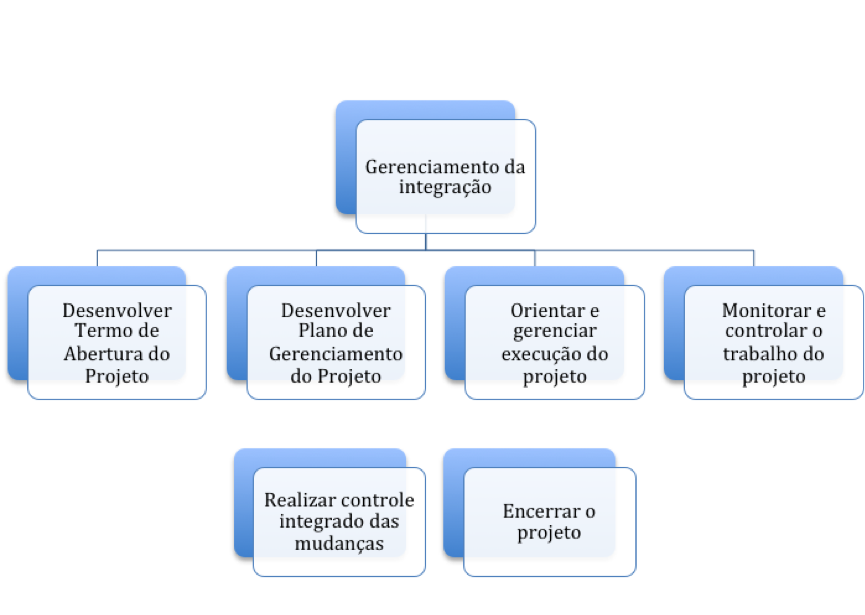
\includegraphics[scale=0.75]{Figuras/gerenciamento_integracao.png}
\caption{Processos do Gerenciamento da Integração}
\label{fig:proc:ger:integr}
\end{figure}

\chapter{Desenvolver o \termo}

O documento chamado de \termo possui três objetivos:

\begin{itemize}
	
	\item Formalmente autorizar um projeto ou uma fase do projeto;
	
	\item Documentar os requisitos iniciais que satisfaçam as necessidades e expectativas das partes interessadas;
	
	\item Estabelecer uma parceria entre a organização executora e a organização solicitante (projetos internos) ou cliente (projetos externos).
	
\end{itemize}

As principais pessoas, organizações ou departamentos envolvidos em sua criação são:

\begin{itemize}
	
	\item[\textbf{\gp}]: dever ser identificado, selecionado e designado o mais cedo possível, preferivelmente enquanto o termo de abertura está sendo desenvolvido e sempre antes do início do planejamento.
	
	\item[\textbf{Patrocinador}]: também chamado de \textit{Sponsor}, é o responsável por assinar a autorização do \termo. Deve ser alguém externo ao projeto e pode ser substituído por um escritório de projetos ou um comitê diretivo de portfólio. Deve estar num nível que seja apropriado para financiá-lo. 
	
\end{itemize}

O processo de desenvolvimento do \termo está representado na Figura \ref{fig:TAP:efts} e será descrito a seguir.

\begin{figure}[!h]
	\centering
	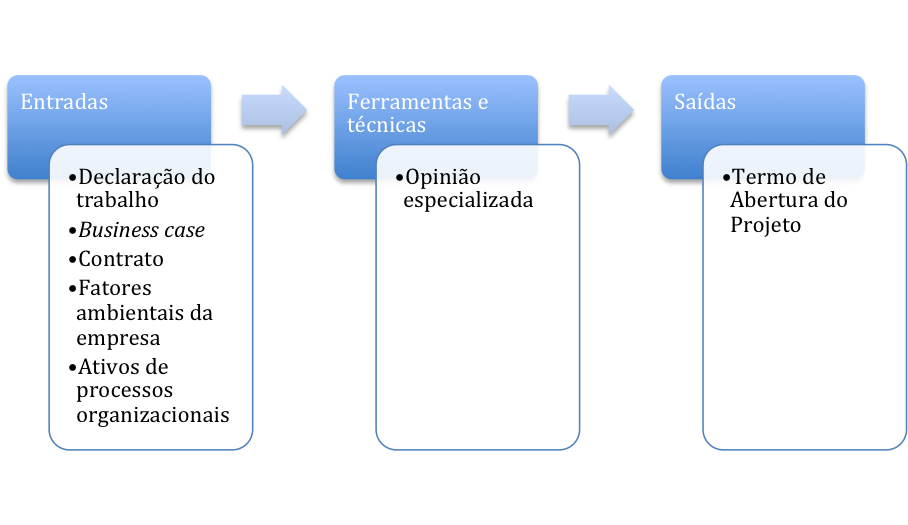
\includegraphics[scale=0.75]{Figuras/TAP_efts.png}
	\caption{Desenvolver o \termo: entradas, ferramentas, técnicas e saídas}
	\label{fig:TAP:efts}
\end{figure}

\section{Entradas}

\begin{itemize}
	
	\item[\textbf{Declaração do trabalho}]: descrição dos produtos e serviços, requisitos necessários das necessidades dos negócios, licitação, proposta, orçamento, etc.
	
	\item[\textbf{\textit{Business Case}}]: fornece informações necessárias, do ponto de vista de um negócio, para determinar se o projeto justifica ou não o investimento. 
	
	\item[\textbf{Contrato}]: quando realizado por um cliente externo.
	
	\item[\textbf{\amb}]: padrões governamentais ou industriais, infraestrutura organizacional e condições de mercado que influenciem no processo.
	
	\item[\textbf{\ativ}]: padrões, políticas e definições padronizadas de processos utilizados na organização, modelos e informações históricas e base de conhecimento de lições aprendidas.
	 
\end{itemize}

\section{Ferramentas e técnicas}

A opinião e especialização é aplicada a qualquer detalhe técnico e de gerenciamento durante esse processo. Pode ser obtida a partir de diversas fontes, inclusive: 

\begin{itemize}
	\item Outras unidades dentro da organização;
	\item Consultores;
	\item Partes interessadas, inclusive clientes ou patrocinadores;
	\item Associações profissionais e técnicas;
	\item Grupos industriais;
	\item Especialistas no assunto e
	\item Escritório de projetos.
\end{itemize}

\section{Saídas}

O \termo deve documentar informações e necessidades, como:

\begin{itemize}
	
 	\item Propósito ou justificativa do projeto;
	
	\item Objetivos mensuráveis do projeto e critérios de sucesso relacionados;
	
	\item Requisitos de alto nível;
	
	\item Descrição do projeto em alto nível;
	
	\item Riscos de alto nível;
	
	\item Resumo do cronograma de marcos;
	
	\item Resumo do orçamento;
	
	\item Requisitos para aprovação do projeto (o que constitui o sucesso do projeto, quem decide se o projeto é bem sucedido, e quem assina o projeto);
	
	\item Gerente do projeto, responsabilidade, nível de autoridade designados e
		
	\item Nome e autoridade do patrocinador ou outra(s) pessoa(s) que autoriza o \termo.
	
\end{itemize}
 
\chapter{Desenvolver o \planproj}
\label{sec:planproj}

É o processo de documentação das ações necessárias para definir, preparar, integrar e coordenar todos os planos auxiliares.

O \planproj tem como objetivos:

\begin{itemize}
	
	\item Auxiliar na gerência do projeto no seu dia a dia;
	
	\item Definir como o projeto é executado, monitorado, controlado e encerrado.
	
\end{itemize}

O documento é formalizado e aprovado pelos \stake e deve conter informações realistas sobre o projeto.

O processo de desenvolvimento do \planproj está representado na Figura \ref{fig:plano:ger:projeto:etfs} e será descrito a seguir.

\begin{figure}[!h]
	\centering
	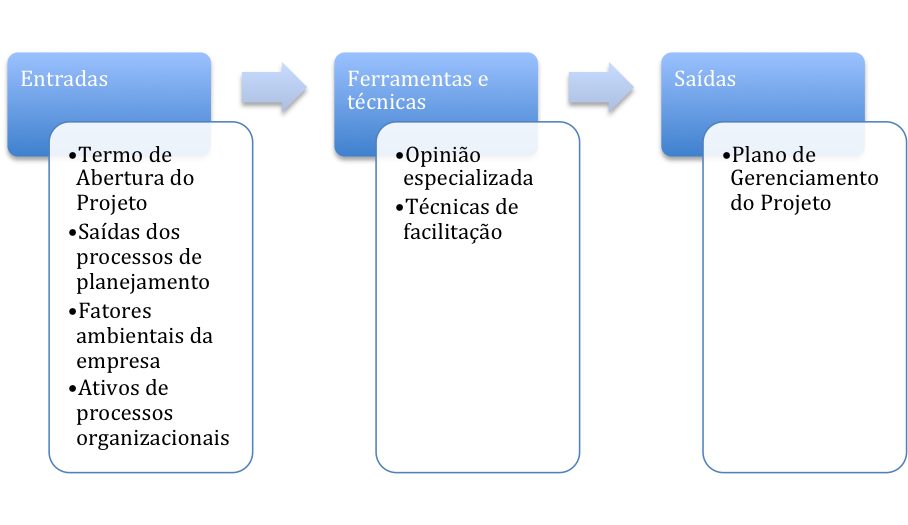
\includegraphics[scale=0.75]{Figuras/plano_ger_projeto_etfs.png}
	\caption{Desenvolver o \planproj: entradas, ferramentas, técnicas e saídas}
	\label{fig:plano:ger:projeto:etfs}
\end{figure}

\section{Entradas}

\begin{itemize}
	
	\item[\textbf{\termo}]: fonte de informações iniciais do projeto.
	
	\item[\textbf{Saídas dos processos de planejamento}]: todos os demais processos de planejamento geram saídas que devem ser integradas para criar o \planproj. Atualizações nestas saídas podem requerer atualizações no \planproj.
	
	\item[\textbf{\amb}]: padrões governamentais ou industriais, sistemas de informações para gerenciamento de projetos, estrutura e cultura organizacionais, infraestrutura e administração de pessoal que influenciem no processo.
	
	
	\item[\textbf{\ativ}]: diretrizes padrão, instruções de trabalho, critérios de avaliação de propostas e critérios de medição de desempenho, modelo de \planproj, procedimentos de controle de mudanças, arquivos de projetos passados, informações históricas e bases de conhecimento de lições aprendidas e bases de conhecimento de gerenciamento de configuração.
	
\end{itemize}

\section{Ferramentas e técnicas}

A opinião especializada é usada para:

\begin{itemize}

	\item Adequar o processo para atender às necessidades do projeto;

	\item Desenvolver detalhes técnicos e de gerenciamento para serem incluídos no \planproj;
	
	\item  Determinar recursos e níveis de habilidades necessárias para executar o trabalho do projeto;
	
	\item Determinar o nível de gerenciamento de configuração a ser usado no projeto e
	
	\item Determinar quais documentos do projeto estarão sujeitos ao processo formal de controle de mudanças.
	
\end{itemize}

As técnicas de facilitação incluem \textit{brainstorming}, resolução de conflitos, solução de problemas e gerenciamento de reuniões.

\section{Saídas}

O \planproj integra e consolida diversos documentos e planos, tais como:

\begin{itemize}

\item[\textbf{Linhas de base do projeto}] : escopo, cronograma e custo.

\item[\textbf{Planos auxiliares de gerenciamento}] : escopo, requisitos, cronograma, custos, qualidade, melhoria de processos, recursos humanos, comunicações, riscos, aquisições e partes interessadas.

\item[\textbf{Processos}] : ciclo de vida selecionado; processos de gerência de projetos, ferramentas e técnicas e como serão adequados ao projeto, níveis de implantacão, em que fases serão utilizados, quais suas dependências, interações, entradas e saídas essenciais.

\item[\textbf{Execução}] : como o trabalho será executado e como as mudanças serão monitoradas e controladas. 

\item[\textbf{Configuração}] : como o gerenciamento de configuração será realizado.

\item[\textbf{Linhas de base}] : como serão mantidas.

\item[\textbf{Partes interessadas}] : necessidades e técnicas para comunicação entre as partes interessadas.

\item[\textbf{Questões em aberto e decisões pendentes}] : revisões chave de gerenciamento do conteúdo, abrangência e melhor momento para facilitar o tratamento.
\end{itemize}

\chapter{Orientar e gerenciar a execução do projeto}

O processo de orientar e gerenciar a execução do projeto está representado na Figura \ref{fig:ori:ger:exe:projeto:etfs} e será descrito a seguir.

\begin{figure}[!h]
	\centering
	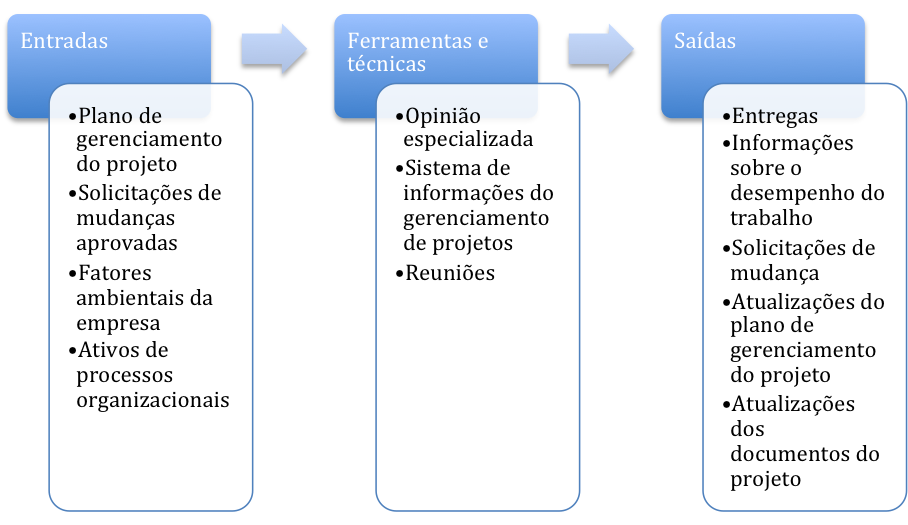
\includegraphics[scale=0.75]{Figuras/ori_ger_exec_proj_efts.png}
	\caption{Orientar e gerenciar a execução do projeto: entradas, ferramentas, técnicas e saídas}
	\label{fig:ori:ger:exe:projeto:etfs}
\end{figure}

\section{Entradas}

\begin{itemize}
	
	\item[\textbf{\planproj}]: planos referentes a todos os aspectos do projeto (ver Seção \ref{sec:planproj}).
	
	\item[\textbf{Solicitações de mudanças aprovadas}]: são agendadas para implementação e podem afetar os planos e documentos do projeto.
	
	\item[\textbf{\amb}]: cultura e estrutura organizacional (da organização ou do cliente), infraestrutura, administração de pessoal, tolerância a riscos das partes interessadas e sistema de informações do gerenciamento de projetos. 
	
	\item[\textbf{\ativ}]: diretrizes padronizadas e instruções de trabalho, requisitos de comunicação que definem os meios de comunicação permitidos, retenção de registros e requisitos de segurança, procedimentos de gerenciamento de questões e defeitos que definem controles de questões e defeitos, identificação e resolução de questões e defeitos, acompanhamento de itens de ação, banco de dados para medição de processos usado para coletar e disponibilizar dados de medição de processos e produtos, arquivos de projetos passados e banco de dados para gerenciamento de questões e defeitos contendo o andamento histórico de questões e defeitos, resolução de questões e defeitos e resultados de itens de ação.
	
\end{itemize}

\section{Ferramentas e técnicas}

\begin{itemize}
	
	\item[\textbf{Opinião especializada}]: orientar e gerenciar a execução do \planproj.
	
	\item[\textbf{Sistema de informações do gerenciamento de projetos}]: ferramentas para automação dos processos.
	
	\item[\textbf{Reuniões}]: troca de informações, \textit{brainstorming}, avaliação de opções e tomada de decisões.
	
\end{itemize}

\section{Saídas}

\begin{itemize}

	\item[\textbf{Entregas}] : produtos e/ou serviços requeridos para completar um processo, fase ou projeto.
	
	\item[\textbf{Informações sobre o desempenho do trabalho}] : indicadores-chave de desempenho, medidas de desempenho técnico, início e fim das atividades agendadas, número de requisições de mudança, número de defeitos, custo real, duração real, etc.
	
	\item[\textbf{Solicitações de mudança}] : proposta formal para modificar qualquer documento, entrega ou linha de base.

	\item[\textbf{Atualizações do \planproj}] :	durante a execução do projeto podem haver atualizações nos elementos que compõe o \planproj.

	\item[\textbf{Atualizações dos documentos do projeto}] : durante a execução do projeto podem haver atualizações nos documentos do projeto.

\end{itemize}

\chapter{Monitorar e controlar o trabalho do projeto}

O processo de monitorar e controlar o trabalho do projeto consiste em acompanhar, revisar e ajustar o progresso para atender aos objetivos de desempenho definidos no plano de gerenciamento. Ele está representado na Figura \ref{fig:mon:cont:trab:projeto:etfs} e será descrito a seguir.

\begin{figure}[!h]
	\centering
	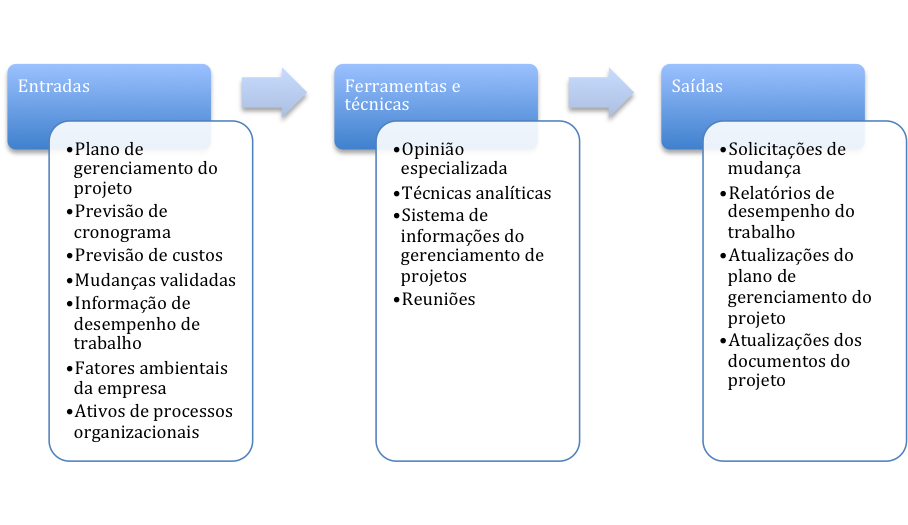
\includegraphics[scale=0.75]{Figuras/mon_cont_trab_efts.png}
	\caption{Monitorar e controlar o trabalho do projeto: entradas, ferramentas, técnicas e saídas}
	\label{fig:mon:cont:trab:projeto:etfs}
\end{figure}

\section{Entradas}

\begin{itemize}
	
	\item[\textbf{\planproj}]: planos referentes a todos os aspectos do projeto (ver Seção \ref{sec:planproj}).
	
	\item[\textbf{\schfor}]: derivado do progresso real versus a linha de base do cronograma.
	
	\item[\textbf{\costfor}]: derivado do progresso real versus a linha de base do custo.
		
	\item[\textbf{Mudanças validadas}]: fornece informações necessárias para confirmar que a mudança foi devidamente executada.
	
	\item[\textbf{Relatórios de desempenho do trabalho}]: dados de desempenho coletados de vários processos de controle, analisados em contexto e integrados de acordo com o relacionamento entre as áreas.
		
	\item[\textbf{\amb}]: padrões governamentais ou industriais, sistema de autorização de trabalho da empresa, tolerância a riscos das partes interessadas e sistema de informações do gerenciamento de projetos. 
	
	\item[\textbf{\ativ}]: requisitos de comunicação da organização, procedimentos de controles financeiros, procedimentos de gerenciamento de questões e defeitos, procedimentos de controle de risco, bancos de dados para medição de processos e bancos de dados de lições aprendidas.
	
\end{itemize}

\section{Ferramentas e técnicas}

\begin{itemize}
	
	\item[\textbf{Opinião especializada}]: usada pela equipe de gerenciamento do projeto para interpretar as informações fornecidas pelos processos de monitoramento e controle.

	\item[\textbf{Técnicas analíticas}]: aplicadas na gerência do projeto para prever potenciais resultados baseado em possíveis mudanças em variáveis do projeto ou de ambiente e sua relação com outras variáveis.
	
	\item[\textbf{Sistema de informações do gerenciamento de projetos}]: ferramentas para automação dos processos.
	
	\item[\textbf{Reuniões}]: inclui a equipe do projeto e outras pessoas interessadas.
	
\end{itemize}

\section{Saídas}

\begin{itemize}
	

	\item[\textbf{Solicitações de mudança}] : podem expandir, ajustar ou reduzir o escopo do projeto ou produto, como resultado das comparações dos resultados planejados com os reais.
	
	\item[\textbf{Relatórios de desempenho do trabalho}] : informações compiladas de documentos do projeto para gerar decisões, ações ou conscientização.

	\item[\textbf{Atualizações do \planproj}] :	durante o controle e monitoramento do projeto podem haver atualizações nos elementos que compõe o \planproj.
	
	\item[\textbf{Atualizações dos documentos do projeto}] : durante o controle e monitoramento do projeto podem haver atualizações nos documentos do projeto.
	
\end{itemize}

\chapter{Realizar o controle integrado de mudanças}

É o processo contínuo de revisar todas as solicitações, aprovar e gerenciar mudanças em entregas, ativos de processos organizacionais, documentos de projeto e \planproj. Ele está representado na Figura \ref{fig:cont:int:mudanca:etfs} e será descrito a seguir.

\begin{figure}[!h]
	\centering
	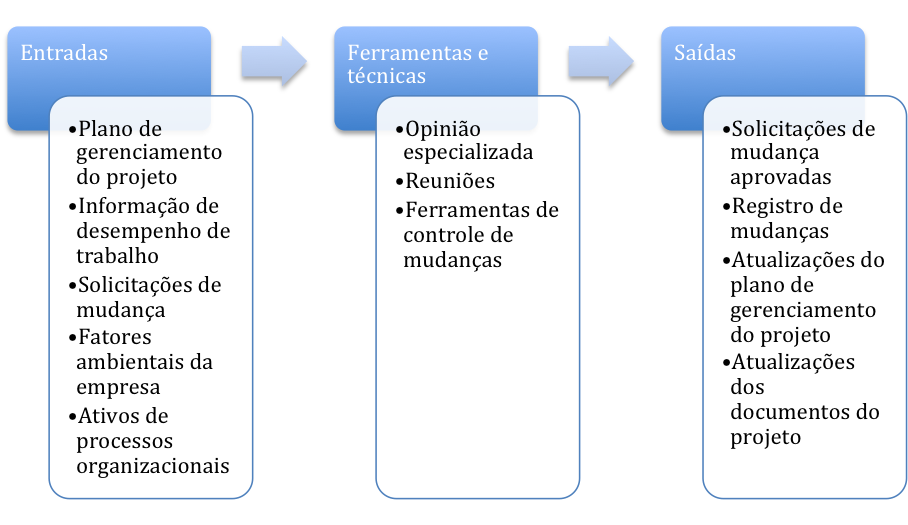
\includegraphics[scale=0.75]{Figuras/cont_int_mudanca_efts.png}
	\caption{Realizar o controle integrado de mudanças: entradas, ferramentas, técnicas e saídas}
	\label{fig:cont:int:mudanca:etfs}
\end{figure}

\section{Entradas}

\begin{itemize}
	
	\item[\textbf{\planproj}]: mudanças são documentadas e atualizadas dentro do \planproj como parte dos processos de gerência de mudanças e configuração.
	
	\item[\textbf{Informação de desempenho de trabalho}]: disponibilidade de recursos, dados de cronograma e custos, análise de valor agregado, gráficos, etc.
	
	\item[\textbf{Solicitações de mudança}]: produzido como saída de diversos processos de monitoramento, controle e execução do projeto.
	
	\item[\textbf{\amb}]: sistema de informações do gerenciamento de projetos. 
	
	\item[\textbf{\ativ}]: procedimentos de controle de mudança, procedimentos para aprovar e endereçar autorizações de mudanças, documentos de projeto, base de conhecimento da gerência de configuração.
	
\end{itemize}

\section{Ferramentas e técnicas}

\begin{itemize}
	
	\item[\textbf{Opinião especializada}]: consultores, partes interessadas (incluindo clientes e o patrocinador), profissionais e técnicos associados, grupos industriais, especialistas e PMO.
	
	\item[\textbf{Reuniões}]: chamadas de reuniões de controle de mudanças, tem como finalidade revisar as solicitações de mudança e aprovar, rejeitar ou dar outras disposições sobre essas mudanças. Quando necessário, um comitê de controle de mudança (\textit{Change Control Board - CCB}) é formado para dirigir as reuniões.
	
	\item[\textbf{Ferramentas de controle de mudanças}]: manuais ou automatizadas, essas ferramentas servem para facilitar a gerência de configuração e mudança.
		
\end{itemize}

\section{Saídas}

\begin{itemize}
	
	
	\item[\textbf{Solicitações de mudança aprovadas}] : serão implementadas através do processo orientar e gerenciar a execução do projeto.
	
	\item[\textbf{Registro de mudanças}] : tem como finalidade documentar as mudanças que ocorrem durante o projeto.
	
	\item[\textbf{Atualizações do \planproj}] :	mudanças podem causar atualizações nos elementos que compõe o \planproj.
	
	\item[\textbf{Atualizações dos documentos do projeto}] : mudanças podem causar atualizações nos documentos do projeto.
	
\end{itemize}


\chapter{nada}

\section{Plano do planejamento}

É considerado como o pré-planejamento. Consiste em atribuir datas, responsáveis e tarefas com o objetivo de planejar o projeto e gerar os documentos e informações necessárias para a \kick. A Figura \ref{fig:plano:planejamento} mostra um exemplo de plano contendo algumas das tarefas mais importantes.

\begin{figure}[!h]
\centering
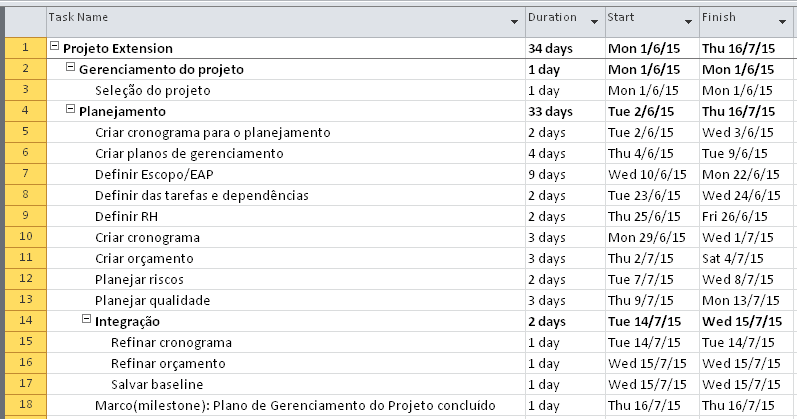
\includegraphics[scale=0.5]{Figuras/plano_planejamento.png}
\caption{Exemplo de Plano do Planejamento}
\label{fig:plano:planejamento}
\end{figure}

\subsection{\Kick}

É o evento que formaliza o início do projeto e que tem como um dos objetivos principais deixar claro os papéis e responsabilidades de todos no projeto. Por isso a participação de todos os \stake é de suma importância. Trata-se de uma ótima oportunidade de colocar frente a frente a equipe, clientes e outros \stake.

\subsection{Integracão dos planos}

Um projeto é como um organismo vivo no qual uma deficiência em uma área pode influenciar uma ou mais outras áreas. Quanto mais tarde essa deficiência for detectada e corrigida, piores serão as consequências.

Por este motivo, os planos de gerenciamento das diversas áreas do projeto não podem ser considerados totalmente independentes e devem ser construídos e mantidos de forma integrada.

Os planos de gerenciamento do projeto seguem as áreas de conhecimento que serão estudadas:

\begin{itemize}

\item \planesc
\item \plancron
\item \plancusto
\item \planqual
\item \planpess
\item \plancom
\item \planrisco
\item \planaq

\end{itemize}

Organizações que possuem escritórios de projeto (PMO) podem definir planos de gerenciamentos padronizados para que não se perca tempo com processos que se repetem em cada novo projeto. Neste caso, cabe ao \gp seguir os processos e planos definidos e o Plano do Planejamento vai incluir somente o cronograma das etapas.

\subsection{Processo Desenvolver o \planproj}

\begin{figure}[!h]
\centering
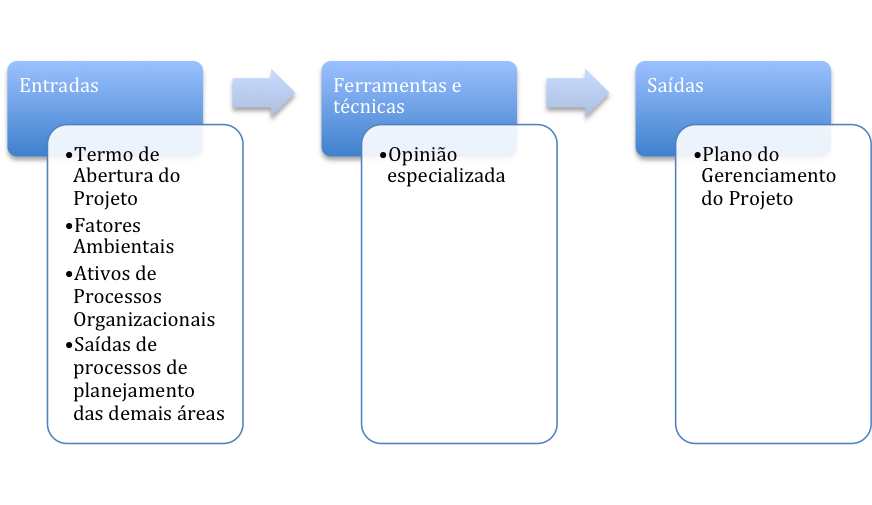
\includegraphics[scale=0.75]{Figuras/proc_integracao_1.png}
\caption{Processo Desenevolver o \planproj}
\label{fig:proc:des:planproj}
\end{figure}

\subsubsection{Entradas}

\begin{itemize}

\item \termo: principal base para início do planejamento, pois possui tudo que ja foi definido para o projeto até o momento.

\item \amb: cultura, infraestrutura, mercado, normas, etc.

\item \ativ: processos e métodos pré-definidos, informações históricas, lições aprendidas, etc.

\item Saidas de processos de planejamento das demais áreas: geram documentos e informações que devem ser integradas para a criação do \planproj. Alterações nestes planos geram alterações no \planproj.

\end{itemize}

\subsubsection{Ferramentas e técnicas}

Opinião especializada:

\begin{itemize}

\item Entender as necessidades do projeto e customizar os processos de acordo

\item Desenvolver e incluir no \planproj detalhes de nível técnico ou gerencial

\item Determinar recursos e conhecimentos necessários para execução do \planproj.

\item Identificar quais documentos necessitam de um processo formal de controle de mudanças.

\end{itemize}

\subsubsection{Saídas}

\planproj.

\subsection{Conteúdo do \planproj}

Além dos demais planos de gerenciamento, o \planproj deve definir:

\begin{itemize}

\item Controle de criação de documentos: quais documentos são necessários, quem tem a responsabilidade de criá-los e quando.

\item Planos auxiliares para gerenciamento das áreas de conhecimento.

\item Linhas de base do escopo, tempo e custo e a formalização dos processos de mudança dessas linhas de base.

\item Processo de controle de mudança:

	\begin{itemize}

	\item Pessoas autorizadas a requisitar mudanças.

	\item Processo de solicitação de mudanças.

	\item Fluxo/processo da mudança:

		\begin{itemize}

		\item Recepção
		\item Análise/avaliação
		\item Classificação
		\item Aprovação
		\item Priorização

		\end{itemize}

\end{itemize}

\end{itemize}
